\documentclass[a4paper,12pt]{report}

% Путь до папки с общими шаблонами
\newcommand{\pathToCommonFolder}{/home/denilai/Desktop/LaTeX/Common}
% Название работы в титуле
\newcommand{\workname}{Отчет по практической работе №3}
% Название дисциплины в титуле
\newcommand{\discipline}{Системное программное обеспечение}
% Название кафедры в титуле
\newcommand{\kafedra}{Кафедра Математического обеспечения и стандартизации информационных технологий}
% Тема работы в титуле
\newcommand{\theme}{Docker}
\newcommand{\rang}{ассистент}
\newcommand{\teacherfio}{Ю.~А.~Вороноцов}




% установка размера шрифта для всего документа
%\fontsize{20pt}{18pt}\selectfont
\usepackage{extsizes} % Возможность сделать 14-й шрифт

\author{Кирилл Денисов}
\title{Практическая работа №3}
\date{\today}

% установка полуторного интервала
% \usepackage{setspace}  
% \onehalfspacing



% Вставка заготовки преамбулы
% Этот шаблон документа разработан в 2014 году
% Данилом Фёдоровых (danil@fedorovykh.ru) 
% для использования в курсе 
% <<Документы и презентации в \LaTeX>>, записанном НИУ ВШЭ
% для Coursera.org: http://coursera.org/course/latex .
% Исходная версия шаблона --- 
% https://www.writelatex.com/coursera/latex/5.3

% В этом документе преамбула

% Для корректного использования русских символов в формулах
% пакеты hyperref и настройки, связанные с ним, стоит загуржать
% перед загрузкой пакета mathtext



% поддержка русских букв
% кодировка шрифта
%\usepackage[T2A]{fontenc} 
\usepackage{pscyr}

% использование ненумеровонного абзаца с добавлением его в содержаниеl

\newcommand{\anonsection}[1]{\section*{#1}\addcontentsline{toc}{section}{#1}}
\newcommand{\sectionunderl}[1]{\section*{\underline{#1}}}


% настройка окружения enumerate
\usepackage{enumitem}
\setlist{noitemsep}
\setlist[enumerate]{labelsep=*, leftmargin=1.5pc}

\usepackage{hyperref}

% сначала ставить \usepackage{extsizes} % Возможность сделать 14-й шрифт
% для корректной установки полей вставлять преамбулу следует в последнюю очередь (но перед дерективой замены \rmdefault)
\usepackage[top=20mm,bottom=25mm,left=35mm,right=20mm]{geometry} % Простой способ задавать поля

\hypersetup{				% Гиперссылки
	unicode=true,           % русские буквы в раздела PDF
	pdftitle={Заголовок},   % Заголовок
	pdfauthor={Автор},      % Автор
	pdfsubject={Тема},      % Тема
	pdfcreator={Создатель}, % Создатель
	pdfproducer={Производитель}, % Производитель
	pdfkeywords={keyword1} {key2} {key3}, % Ключевые слова
	colorlinks=true,       	% false: ссылки в рамках; true: цветные ссылки
	linkcolor=red,          % внутренние ссылки
	citecolor=black,        % на библиографию
	filecolor=magenta,      % на файлы
	urlcolor=blue           % на URL
}

%%% Работа с русским языком
\usepackage{cmap}					% поиск в PDF
\usepackage{mathtext} 				% русские буквы в формулах
\usepackage[T2A]{fontenc}			% кодировка
\usepackage[utf8]{inputenc}			% кодировка исходного текста
\usepackage[english,russian]{babel}	% локализация и переносы
\usepackage{indentfirst}
\frenchspacing

%для изменения названия списка иллюстраций
\usepackage{tocloft}


\renewcommand{\epsilon}{\ensuremath{\varepsilon}}
\renewcommand{\phi}{\ensuremath{\varphi}}
\renewcommand{\kappa}{\ensuremath{\varkappa}}
\renewcommand{\le}{\ensuremath{\leqslant}}
\renewcommand{\leq}{\ensuremath{\leqslant}}
\renewcommand{\ge}{\ensuremath{\geqslant}}
\renewcommand{\geq}{\ensuremath{\geqslant}}
\renewcommand{\emptyset}{\varnothing}

% Изменения параметров списка иллюстраций
\renewcommand{\cftfigfont}{Рисунок } % добавляем везде "Рисунок" перед номером
\addto\captionsrussian{\renewcommand\listfigurename{Список иллюстративного материала}}

\newcommand{\tm}{\texttrademark\ }
\newcommand{\reg}{\textregistered\ }


%%% Дополнительная работа с математикой
\usepackage{amsmath,amsfonts,amssymb,amsthm,mathtools} % AMS
\usepackage{icomma} % "Умная" запятая: $0,2$ --- число, $0, 2$ --- перечисление

%% Номера формул
%\mathtoolsset{showonlyrefs=true} % Показывать номера только у тех формул, на которые есть \eqref{} в тексте.
%\usepackage{leqno} % Нумереация формул слева

%% Свои команды
\DeclareMathOperator{\sgn}{\mathop{sgn}}

%% Перенос знаков в формулах (по Львовскому)
\newcommand*{\hm}[1]{#1\nobreak\discretionary{}
{\hbox{$\mathsurround=0pt #1$}}{}}


% отступ для первого абзаца главы или параграфа
%\usepackage{indentfirst}

%%% Работа с картинками
\usepackage{graphicx}  % Для вставки рисунков
\graphicspath{{images/}{screnshots/}}  % папки с картинками
\DeclareGraphicsExtensions{.pdf,.png,.jpg}
\setlength\fboxsep{3pt} % Отступ рамки \fbox{} от рисунка
\setlength\fboxrule{1pt} % Толщина линий рамки \fbox{}
\usepackage{wrapfig} % Обтекание рисунков текстом

%%% Работа с таблицами
\usepackage{array,tabularx,tabulary,booktabs} % Дополнительная работа с таблицами
\usepackage{longtable}  % Длинные таблицы
\usepackage{multirow} % Слияние строк в таблице

%%% Теоремы
\theoremstyle{plain} % Это стиль по умолчанию, его можно не переопределять.
\newtheorem{theorem}{Теорема}[section]
\newtheorem{proposition}[theorem]{Утверждение}

\theoremstyle{plain} % Это стиль по умолчанию, его можно не переопределять.
\newtheorem{work}{Практическая работа}[part]


 
 
\theoremstyle{definition} % "Определение"
\newtheorem{corollary}{Следствие}[theorem]
\newtheorem{problem}{Задача}[section]
 
\theoremstyle{remark} % "Примечание"
\newtheorem*{nonum}{Решение}



%%% Программирование
\usepackage{etoolbox} % логические операторы

%%% Страница

%	\usepackage{fancyhdr} % Колонтитулы
% 	\pagestyle{fancy}
%   \renewcommand{\headrulewidth}{0pt}  % Толщина линейки, отчеркивающей верхний колонтитул
% 	\lfoot{Нижний левый}
% 	\rfoot{Нижний правый}
% 	\rhead{Верхний правый}
% 	\chead{Верхний в центре}
% 	\lhead{Верхний левый}
%	\cfoot{Нижний в центре} % По умолчанию здесь номер страницы

\usepackage{setspace} % Интерлиньяж
\onehalfspacing % Интерлиньяж 1.5
%\doublespacing % Интерлиньяж 2
%\singlespacing % Интерлиньяж 1

\usepackage{lastpage} % Узнать, сколько всего страниц в документе.

\usepackage{soul} % Модификаторы начертания


\usepackage[usenames,dvipsnames,svgnames,table,rgb]{xcolor}


\usepackage{csquotes} % Еще инструменты для ссылок

%\usepackage[style=authoryear,maxcitenames=2,backend=biber,sorting=nty]{biblatex}

\usepackage{multicol} % Несколько колонок

\usepackage{tikz} % Работа с графикой
\usepackage{pgfplots}
\usepackage{pgfplotstable}

% модуль для вставки рыбы
\usepackage{blindtext}

\usepackage{listings}
\usepackage{color}


% для поворота отдельной страницы. Использовать окружение \landscape
\usepackage{pdflscape} 
\usepackage{rotating} 


\definecolor{mygreen}{rgb}{0,0.6,0}
\definecolor{mygray}{rgb}{0.5,0.5,0.5}
\definecolor{mymauve}{rgb}{0.58,0,0.82}


% пример импорта файла
%\lstinputlisting{/home/denilai/repomy/conf/distributions}

\lstset{
	language=Python,
	basicstyle=\footnotesize,        % the size of the fonts that are used for the code
	numbers=left,                    % where to put the line-numbers; possible values are (none, left, right)
	numbersep=5pt,                   % how far the line-numbers are from the code
	numberstyle=\tiny\color{mygray}, % the style that is used for the line-numbers
	stepnumber=2,                    % the step between two line-numbers. If it's 1, each line will be numbered
	% Tab - 2 пробела
	tabsize=2,    
	% Автоматический перенос строк
	breaklines=true,
	frame=single,
	breakatwhitespace=true,
	title=\lstname 
}



% использовать Times New Roman
\renewcommand{\rmdefault}{ftm}

\begin{document}

	%\thispagestyle{empty}
	
	% Вставка первого титульного листа
	%%\newcounter{withouttheme}

%\setcounter{withouttheme}{<n>} установить значение счетчика  withouttheme для определения, нужна ли тема
%    {0} - нужна
%    {1} - не нужна

%\setcounter{withoutsubmissiondate}{<n>} установить значение счетчика  withoutsubmissiondate для определения, нужна ли дата представления к защите
%     {0} - нужна
%     {1} - не нужена
\begin{center}
	\begin{figure}[h!]
		\begin{center}
		%\vspace{-10ex}
		
\includegraphics[width=0.17\linewidth]{\pathToCommonFolder/gerb}
		%\caption{}\label{pic:first}
		%	\vspace{5ex}
		\end{center}	
	\end{figure}
 	\small	МИНОБРНАУКИ РОССИИ \\
	Федеральное государственное бюджетное образовательное учреждение\\
						высшего образования\\
\normalsize					
\textbf{«МИРЭА – Российский технологический университет»\\
						РТУ МИРЭА}\\
						\noindent\rule{1\linewidth}{1pt}\\
       Институт информационных технологий\\ %\vspace{2ex}
					\kafedra\\
		\vspace{3ex}
			\large \textbf{\workname}  \\
		%\vspace{1ex}
						по дисциплине\\ «\discipline» \\
		\vspace{3ex}
		\ifnum \value{withouttheme}=0 {
			\textbf{Тема работы:}\\ <<\theme>>
		}
		\else {}
		\fi
\vspace{10ex}
\small
\begin{table}[h!]
\begin{tabular}{lp{0.6\linewidth}l}
	\textbf{Выполнил:} & студент группы ИВБО-02-19 & \\ 
	& & \studentfio \\%Д.~Н.~Федосеев\\%А.~М.~Сосунов\\%К.~Ю.~Денисов\\%И.~А.~Кремнев
	\textbf{Принял:} & \rang & \\
	& & \teacherfio \hfill\\
\end{tabular}
\end{table}
\end{center}
\ifnum \value{withoutsubmissiondate}=0 {
	\begin{flushleft}
		Работа представлена к защите <<\rule{3ex}{1pt}>>\rule{10ex}{1pt} 202\rule{1ex}{1pt} г.\hfill
	\end{flushleft}
\else {}
\fi

\normalsize
\begin{center}	
\vfill
Москва 2022
\end{center}

	
	\newpage
	\tableofcontents
	\newpage
	
	
\chapter{Краткий обзор StarUML}

StarUML\tm --- программный инструмент моделирования, который поддерживает UML
(Унифицированный язык моделирования). StarUML ориентирован на UML версии 1.4 и
поддерживает одиннадцать различных типов диаграмм, принятых в нотации UML 2.0. Он активно
поддерживает подход MDA (Модельно-управляемая архитектура), реализуя концепцию профилей
UML. Среда разработки StarUML\tm превосходно настраивается в соответствии с требованиями
пользователя и имеет высокую степень расширяемости, особенно в области своих
функциональных возможностей. Использование StarUML\tm, одного из ведущих программных
инструментов моделирования, гарантирует достижение максимальной производительности и
качества ваших программных проектов.
\subsection*{Инструмент UML, который адаптируется к пользователю}
StarUML\tm  предоставляет максимальную степень адаптации среды разработки пользователя,
предлагая настройку параметров, которые могут влиять на методологию разработки программного
обеспечения, проектную платформу и язык.

\subsection*{Превосходная расширяемость и гибкость}
StarUML\tm  обеспечивает превосходную расширяемость и гибкость. Он предоставляет механизм
аддинов, чтобы расширять свои функциональные возможности. Этот механизм разработан
специально, чтобы предоставлять доступ ко всем функциям модели/мета-модели посредством
COM Automation и расширять меню и набор свойств элементов. Также, пользователи могут
создавать собственные подходы и механизмы согласно своим собственным методологиям.
Программа может также быть интегрирована с любыми внешними инструментальными
средствами.

\subsection*{Системные требования}
Ниже указаны минимальные системные требования, необходимые для функционирования
StarUML\tm.
\begin{itemize}
	\item Intel \reg Pentium \reg 233MHz или выше
	\item Windows \reg 2000, Windows XP TM, или выше
	\item Microsoft \reg Internet Explorer 5.0 или выше
	\item 128 Мбайт RAM (256 МБ рекомендуется)
	\item 110 Мбайт на жестком диске (150 МБ рекомендуется)
	\item Устройство CD-ROM
	\item SVGA или монитор с более высокой разрешающей способностью (1024x768 рекомендуется)
	\item Мышь или другое устройство позиционирования
\end{itemize}
\chapter{Основные концепции}
Эта глава вводит фундаментальные концепции, которые требуется знать для эффективного
использования StarUML\tm. Она содержит описание моделей, визуальных элементов и диаграмм,
проектов, секций, подходов, фреймворков, модельных фрагментов, их различий относительно
разных профилей UML.
\begin{itemize}
	\item Модель,
	\item Представление (view) и Диаграмма
	\item Проект и проектная секция (unit)
	\item Модуль (module)
\end{itemize}

\sectionunderl{Модель, Представление и Диаграмма}
% TODO: \usepackage{graphicx} required
\begin{figure}[h!]
	\centering
	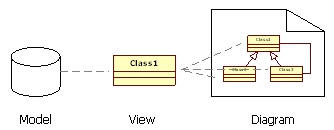
\includegraphics[width=0.7\linewidth]{images/modelviewdiagram}
	\caption{Модель, представление, диаграмма}
	\label{fig:modelviewdiagram}
\end{figure}
StarUML\tm предполагает ясное понимание концептуального различия между моделями,
представлениями и диаграммами. Модель --- элемент, который содержит всю информацию о модели
программы. Представление --- визуальное выражение информации, содержавшейся в модели, а
Диаграмма --- коллекция визуальных образов, которая отображает определенные аспекты проекта.

\sectionunderl{Проект и проектная секция}
\subsubsection*{Проект}
Проект -- основная структурная единица в StarUML\tm.
Проект может содержать одну или более программных моделей. Проект - корневой пакет
верхнего уровня, который всегда существует в любой программной модели. В общем случае, один
проект сохраняется в одном файле.

\subsubsection*{Структура проекта}
Проект содержит следующие суб-элементы:

Модель --- элемент, который соответствует одной программной модели.

Подсистема --- элемент, который соответствует модели подсистемы.

Пакет --- самый общий элемент для группировки других элементов.

\subsubsection*{Проектный файл}Проектные файлы сохраняются в формате XML и имеют расширение \textit{".UML"}. Все модели,
представления и диаграммы, созданные в StarUML\tm сохраняются в одном проектном файле.
Проект может также быть разделен и сохранен в нескольких проектных секциях. Проектный файл
содержит следующую информацию:
\begin{itemize}
	\item профиль UML, используемый в проекте
	\item файлы секций, на которые ссылается проект
	\item информация по всем моделям, содержавшимся в проекте
	\item информация по всем диаграмм и представлениям, содержавшимся в проекте
\end{itemize}
\

\chapter{Управление проектом}
Эта глава подробно описывает операции по управлению проектом: создание нового проекта,
размещение части проекта в секции, создание и импорт фрагментов модели, импорт фреймворков,
подключение и исключение профилей UML.
\begin{itemize}
	\item Управление проектом
	\item Управление секциями
	\item Работа с фрагментами модели
	\item Импорт фреймворка
	\item Работа с профилями UML
\end{itemize}

\sectionunderl{Управление проектом}
\subsection*{Создание нового проекта}
Чтобы начать разработку программного обеспечения, нужно инициировать новый проект. Вы
можете начать абсолютно пустой проект или инициализировать новый проект согласно
определённому подходу.

\subsubsection*{Процедура создания нового проекта \#1 --- New Project:}
\begin{enumerate}
	\item выберите меню [File] -> [New Project].
	\item Новый проект будет создан в соответствии с подходом по умолчанию, ранее выбранным
	пользователем. В зависимости от подхода могут быть подгружены определённые профили
	и/или инструментарии.
\end{enumerate}
 
\subsubsection*{Процедура создания нового проекта \#2 --- Select Select New Project}
\begin{enumerate}
	\item Выберите меню [File] -> [Select New Project...].
	диалоговом окне New Project будет отображен список доступных подходов.
	\item Выберите	нужный из списка и нажмите кнопку [OK].
	\item Новый проект будет создан и инициализирован согласно указанному подходу. В
	зависимости от подхода могут быть подгружены определённые профили и/или фреймворки.
\end{enumerate}
% TODO: \usepackage{graphicx} required
\begin{figure}[h!]
	\centering
	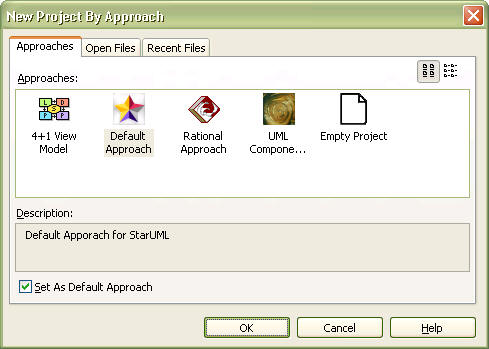
\includegraphics[width=0.7\linewidth]{images/newproject}
	\caption{Новый проект}
	\label{fig:newproject}
\end{figure}

\paragraph{Примечание}
\begin{itemize}
	\item Список доступных подходов зависит от инсталлированной среды разработки пользователя.
	\item Чтобы изменить заданный по умолчанию подход, откройте диалоговое окно "Select New
	Project", выберите нужный подход и затем установите опцию "Set As Default Approach"
	(Использовать как подход по умолчанию).
\end{itemize}

\subsection*{Открытие проекта}
Чтобы начать работать с существующим проектом, его проектный файл нужно открыть. Если
проект включает более одной секции, все связанные секции будут также загружены вместе с
проектом.

\subsubsection*{Процедура открытия проекта:}
\begin{enumerate}
	\item Выберите меню [File] -> [Open...].
	\item В диалоговом окне "Open Project", выберите файл проекта (.UML) и нажмите кнопку
	[Open].
	\item Выбранный проектный файл будет открыт.
\end{enumerate}

\paragraph{Примечание}
Проекты могут также быть открыты через диалоговое окно "Select New Project".

\subsection*{Сохранение проекта}
Чтобы изменения, сделанные в проекте, не пропали, проектный файл должен быть должным
образом сохранен. Ваша работа может быть сохранена в существующий проектный файл или в 
новый проектный файл. Когда проектный файл сохраняется, то вместе с ним сохраняются данные
из связанных с ним секций.
\subsubsection*{Процедура сохранения проекта:}
\begin{enumerate}
	\item Выберите меню [File] -> [Save].
	\item Если имя файла проекта не было определено, появится диалоговое окно "Save Project".
	Введите имя файла, и нажмите кнопку [Save].
	\item Проектный файл будет сохранен.
\end{enumerate}
% TODO: \usepackage{graphicx} required
\begin{figure}[h!]
	\centering
	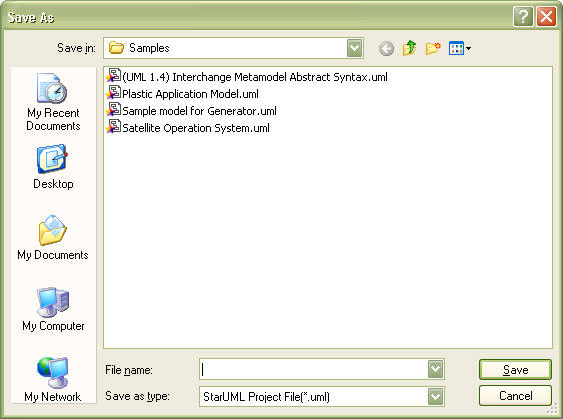
\includegraphics[width=0.7\linewidth]{images/saveproject}
	\caption{Сохранение проекта}
	\label{fig:saveproject}
\end{figure}


\subsubsection*{Процедура сохранения проекта в новом файле:}
\begin{enumerate}
	\item Выберите меню [File] -> [Save As...].
	\item В диалоговом окне "Save As", введите новое имя файла, и нажмите кнопку [Save].
	\item Проект будет сохранен в указанном файле.
\end{enumerate}

\paragraph{Примечание}
\begin{itemize}
	\item Если проект содержит одну или более секций, и есть изменённые секции, диалоговое окно
	будет запрашивать подтверждение на сохранение каждой измененной секции. Выберите
	[Yes], чтобы сохранить измененную секцию вместе с проектом.
\end{itemize}

\subsection*{Закрытие проекта}
Проект может быть закрыт, если больше не требуется его редактирование.
\subsubsection*{Процедура закрытия проекта:}
\begin{enumerate}
	\item Выберите меню [Файл]->[Close].
	\item Если проект не был сохранен после внесения изменений, пользователю будет предложено
	сохранить изменения. Пользователь может выбрать <<да>>, <<нет>> или <<отмена>>.
	\item После закрытия проект становится недоступным для редактирования.
\end{enumerate}
\begin{figure}[h!]
	\centering
	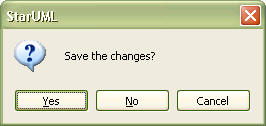
\includegraphics[width=0.7\linewidth]{images/closeproject1}
	\caption{Сохранение изменений}
	\label{fig:closeproject1}
\end{figure}


\subsection{Управление элементами с помощью моделей, подсистем и пакетов}
Программная модель состоит из многих элементов и диаграмм. Правильная группировка этих
элементов и диаграмм очень важна для эффективного управления проектом. StarUML\tm
поддерживает три типа группирующих элементов (модели, подсистемы и пакеты), которые
пользователь может использовать соответственно их назначению.
Способы группировки элементов, реализованные в StarUML\tm
\newpage

\includegraphics[width=3ex]{images/folder}Модель

Модель выражает физическую систему в определенном аспекте. Например, это может быть аспект
анализа, аспект проекта, пользовательский аспект, и т.д.

% TODO: \usepackage{graphicx} required

\includegraphics[width=3ex]{images/subsistem}
Подсистема

Подсистема группирует элементы, которые составляют полную физическую систему или её части.

% TODO: \usepackage{graphicx} required

\includegraphics[width=3ex]{images/package}
Пакет

Пакет логически группирует и содержит модельные элементы. Это чрезвычайно обобщенный
элемент, который может использоваться только для того, чтобы как-то организовать модельные
элементы.

\chapter{Моделирование с помощью StarUML}
Эта глава подробно описывает, как создавать и редактировать элементы диаграммы, включая
способы организации структуры модели с помощью навигатора модели.
\begin{itemize}
	\item Редактирование элементов и диаграмм
	\item Организация структуры модели
\end{itemize}

\sectionunderl{Редактирование элементов и диаграмм}
\subsection*{Создание новой диаграммы}
StarUML TM поддерживает 11 типов диаграмм UML. Пользователь может свободно создавать и
манипулировать диаграммами различных типов, как ему необходимо.
\subsubsection*{Процедура создания новой диаграммы:}
\begin{enumerate}
	\item Выберите в навигаторе модели или на диаграмме элемент, который будет содержать новую
	диаграмму.
	\item Щелкните правой кнопкой мыши и выберите [Add Diagram]. Новая диаграмма будет
	создана после выбора типа диаграммы.
\end{enumerate}

\subsubsection*{Доступные типы диаграмм}
\begin{itemize}
 
\item \textbf{Диаграмма классов (Сlass diagram)}

Диаграмма классов - визуальное отображение различных статических отношений между
класс-подобными элементами. Диаграмма классов может содержать не только классы, но
также и интерфейсы, перечислимые типы, пакеты, различные отношения, инстанции и их
связи.
\item \textbf{Диаграмма прецедентов (Use case diagram)}

Диаграмма прецедентов - отображение отношений между вариантами использования
(прецедентами) определенной системы или объекта и внешними акторами. Вариант
использования отображает функции системы и то, как эти функции взаимодействуют с
внешними акторами.
\item \textbf{Диаграмма сообщений (Sequence Diagram)}

Диаграмма сообщений отображает взаимодействие инстанций. Она является прямым отображением множества взаимных воздействий (InteractionInstanceSet) между элементами
множества инстанций (CollaborationInstanceSet). В то время как Диаграмма сообщений роли
ориентирована на классификаторы-роли, обычная Диаграмма сообщений - на инстанции.
\item \textbf{Диаграмма сообщений роли (Sequence Role Diagram)}

Диаграмма сообщений роли отображает взаимодействия в концепции ролей. Она является
прямым отображением Interaction (множества взаимных сообщений между
классификаторами-ролями) в пределах Collaboration. В то время как Диаграмма сообщений
- отображение инстанций, Диаграмма сообщений роли - отображение классификаторов-
ролей.
\item \textbf{Диаграмма коллаборации (Collaboration Diagram)}

 Диаграмма коллаборации отображает взаимодействие между инстанциями. Она является
прямым отображением модели взаимодействия инстанций, входящих в CollaborationInstanceSet. В то время как диаграмма коллаборации ролей - отображение
классификаторов-ролей, обычная диаграмма коллаборации - отображение инстанций.
\item \textbf{Диаграмма коллаборации ролей}

Диаграмма коллаборации ролей отображает взаимодействия между ролями. Она является
прямым отображением модели взаимодействия классификаторов-ролей внутри
коллаборации. В то время как обычная диаграмма коллаборации ориентирована на
отображение инстанций, диаграмма коллаборации ролей - отображение классификаторов-
ролей.
\item\textbf{ Диаграмма состояний (Statechart Diagram)}

Диаграмма состояний выражает статическое поведение определенного объекта через
состояния и переходы состояний. Хотя диаграмма состояний обычно используется, чтобы
выразить поведение инстанций классов, она может также использоваться, чтобы выражать
поведение и других элементов.
\item \textbf{Диаграмма действий (Activity Diagram)}

Диаграмма действий - специальная форма диаграммы состояний, которая является
подходящей для того, чтобы отображать поток выполнения действий. Диаграмма действий в
общем случае используется для отображения любых потоков обработки, но чаще всего
применительно к объектам подобным классам, пакетам и операциям.
\item \textbf{Диаграмма компонентов (Component Diagram)}

Диаграмма компонентов отображает зависимость между программными компонентами.
Элементы, которые составляют программные компоненты и элементы, которые реализуют
эти компоненты, могут быть отображены на диаграмме компонентов.
\item \textbf{Диаграмма развертывания (Deployment Diagram)}

Диаграмма развертывания отображает аппаратные элементы компьютера, другие
устройства и программные компоненты, а также процессы и объекты, которые им
назначены.
\item \textbf{Композиционная структурная диаграмма (Composite Structure Diagram)}

Композиционная структурная диаграмма - диаграмма, выражающая внутреннюю структуру
классификатора. Она показывает его точки зрения взаимодействия с другими частями
системы.

\end{itemize}
\paragraph*{Примечание}
\begin{itemize}
	\item Типы доступных диаграмм изменяются при переходе от одного типа элемента к другому.
\end{itemize}
\subsection*{Создание элемента на диаграмме}
Чтобы создать на диаграмме новый элемент, диаграмму сначала нужно открыть. Палитра
элементов содержит различные типы элементов, доступных для создания в зависимости от типа
диаграммы. Список доступных элементов изменяется при переходе от диаграммы одного типа к
диаграмме другого типа.


\subsubsection*{Процедура создания элемента из палитры элементов:}
\begin{enumerate}
	\item Выберите тип создаваемого элемента на палитре элементов.
	\item Щёлкните желаемое место для нового элемента на диаграмме, чтобы создать там элемент.
	(Перетаскивайте указатель мыши, чтобы определить область и размер нового элемента. При
	создании элемента, который соединяет два других элемента, убедитесь, что соединение
	сделано правильно.)
\end{enumerate}

\subsubsection*{Процедура одновременного создания нескольких однотипных элементов:}
\begin{enumerate}
	\item Выберите тип создаваемого элемента на палитре элементов.
	\item Нажмите [Lock] на палитре или тот же тип элемента еще раз.
	\item Создайте несколько элементов подряд.
	\item Снова нажмите элемент в палитре, когда создание группы элементов будет закончено.
\end{enumerate}

\paragraph{Примечание}
\begin{itemize}
	\item Создание элемента на диаграмме с помощью палитры элементов фактически означает
	создание как собственно модельного элемента, так и его визуального образа.
\end{itemize}


\subsection*{Редактирование элемента на диаграмме}
Элементы могут редактироваться непосредственно на диаграмме.
\subsubsection*{Процедура редактирования элемента:}
\begin{enumerate}
	\item Дважды щелкните образ на диаграмме.
	\item В "горячем диалоге" редактируйте имя элемента, область видимости и т.д., или нажмите
	кнопку, чтобы создать подчинённые элементы для выбранного элемента.
	\item Нажмите [Enter] или щёлкните другое место на диаграмме, чтобы принять изменения.
\end{enumerate}

\paragraph{Примечание}
\begin{itemize}
	\item Для детального описания работы с горячим диалогом, см. Горячие диалоги.
	
\end{itemize}

\subsection*{Изменение размеров и перемещение}
Вы можете оптимизировать размер визуального образа и его позицию внутри диаграммы, а
также Вы можете плавно менять его позицию и устанавливать размеры комбинацией клавиш
<Специальная>+<Клавиша курсора>.

\subsubsection*{Процедура изменения размера образа:}
\begin{enumerate}
	\item  Щёлкните образ на диаграмме.
	\item Изменяйте размер образа перетаскиванием в нужном направлении одного из маркеров, которые показываются после выделения образа.
\end{enumerate}

\subsubsection*{Процедура изменения размеров образа, используя клавиатуру:}
\begin{enumerate}
	\item Выделите образ, щёлкнув его на диаграмме.
	\item Для изменения размеров образа пользователь может применить комбинацию Shift +Cusor
	key. Эта комбинация обеспечивает изменение шагами установленного размера, но Вы
	можете изменять размер образа плавно комбинацией Shift +Alt+Cursor.
\end{enumerate}

\subsubsection*{Процедура перемещения образа:}
\begin{enumerate}
	\item Выделите передвигаемый образ щёлкнув его на диаграмме. Если нужно выделить несколько
	образов, выделяйте их комбинацией Shift+Click или очертите мышью область на диаграмме.
	\item Переместите образы в нужное место перетаскиванием, используя мышь.
\end{enumerate}



\subsubsection*{Процедура перемещения образа, используя клавиатуру:}
\begin{enumerate}
	\item Выделите передвигаемый образ щёлкнув его на диаграмме. Если нужно выделить несколько
	образов, выделяйте их комбинацией Shift+Click или очертите мышью область на диаграмме.
	\item Переместите образы куда нужно, используя Ctrl+Cursor Key. Эта комбинация обеспечивает
	передвижение шагами установленного размера, но Вы можете передвигать образ плавно
	комбинацией Ctrl+Alt+Cursor Key.
\end{enumerate}


\subsection*{Создание элемента с использованием "горячего синтаксиса"}
Элементы также могут быть созданы без использования мыши, использованием горячего
синтаксиса.
\subsubsection*{Процедура создания элемента с помощью горячего синтаксиса:}
\begin{enumerate}
	\item Выберите образ на диаграмме.
	\item Вызовите горячий диалог, нажав [Enter].
	\item Введите нужный синтаксис в горячем диалоге.
\end{enumerate}

\subsubsection*{Горячий синтаксис генерации}
Горячий синтаксис позволяет генерировать элементы модели и отношения через написание
несложного текста. Основное правило горячего синтаксиса состоит в следующем. Напишите имя
целевого модельного элемента и установленный нотационный знак, чтобы создать отношение
соответствующее этому знаку между текущим и целевым элементом. Если целевое имя не указано,
будет сгенерирован новый модельный элемент и указанное отношение. Нотация знаков отношений горячего синтаксиса приведена ниже:




\end{document}
